\documentclass{article}
\usepackage{graphicx} % Required for inserting images
\usepackage{kotex}
\usepackage{caption}
\usepackage{subcaption}

\title{프로그래밍언어론 HW 0}
\date{2024. 03. 15.}

\begin{document}

\maketitle
\section{자기소개}
이름: 권찬\newline
전공: 컴퓨터공학과\newline
학번: C011013

\section{수식작성}
극한값의 계산\newline
수열의 극한에 대한 기본 성질\\
수열 $\{a_n\}, \{b_n\}$이 모두 수렴하고,\\
$\lim\limits_{n\to\infty} a_n  = \alpha, \lim\limits_{n\to\infty} b_n = \beta$ 일 때,\\\\
- $\lim\limits_{n\to\infty} ca_n  = c\lim\limits_{n\to\infty} a_n = c\alpha$\\
- $\lim\limits_{n\to\infty} (a_n + b_n)  = \alpha + \beta$\\
- $\lim\limits_{n\to\infty} (a_n - b_n)  = \alpha - \beta$\\
- $\lim\limits_{n\to\infty} a_n b_n = \lim\limits_{n\to\infty} a_n \lim\limits_{n\to\infty} b_n = \alpha \beta$\\
- $\lim\limits_{n\to\infty} \frac{a_n}{b_n} = \frac{\lim\limits_{n\to\infty} a_n}{\lim\limits_{n\to\infty} a_n} =\frac{\alpha}{\beta}$\\
(단, $b_n \neq 0, \beta \neq 0$)\\
$\lim\limits_{n\to\infty} \frac{1}{n} = 0$
\newpage
\section{가장 좋아하는 그림}
\begin{figure}[!htb]
    \centering
    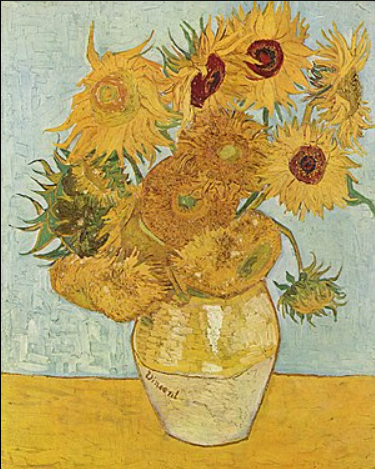
\includegraphics[width=0.5\linewidth]{image1.png}
    \caption{반 고흐의 해바라기}
    \label{fig-1}
\end{figure}
\begin{figure}[!htb]
    \centering
    \begin{subfigure}[!htb]{0.4\textwidth}
        \centering
        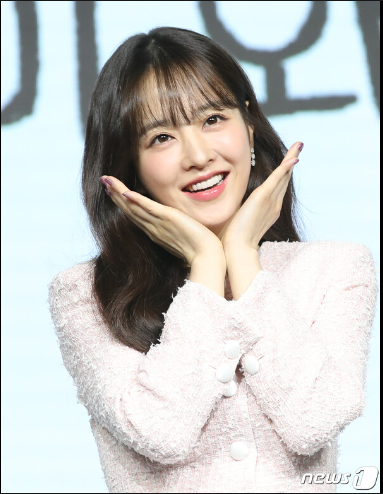
\includegraphics[width=0.5\linewidth]{image2.png}
        \caption{사진1}
        \label{fig:fig-2-a}
    \end{subfigure}
    \hfill
    \begin{subfigure}[!htb]{0.4\textwidth}
        \centering
        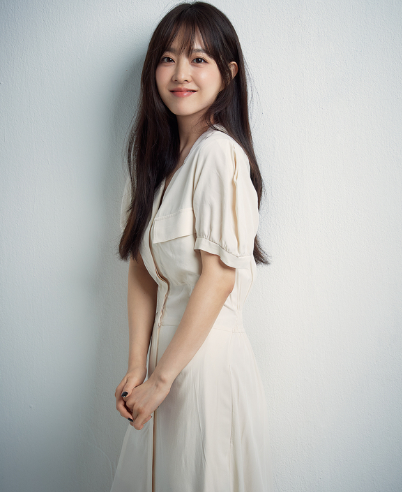
\includegraphics[width=0.5\linewidth]{image.png}
        \caption{사진2}
        \label{fig:fig-2-b}
    \end{subfigure}
    \caption{대한민국 배우 박보영}
    \label{fig:fig-2}
\end{figure}
    \subsection{자신을 나타낼 수 있는 사진}
    Figure~\ref{fig-1}에서 보는 것같이 나는 해바라기처럼 좋아하는 것을 적극적으로 쫓는 사람이다.
    \subsection{좋아하는 연예인 사진}
    Figure~\ref{fig:fig-2}에서 보는 것과 같이 배우 박보영을 좋아한다.

\section{참고 문헌}
인용 확인~\cite{floridi2020gpt}
\bibliographystyle{plain}
\bibliography{hw0}
\end{document}
